\chapter{Implementation and Testing}\label{chap:implementation}

This chapter provides the implementation details of the DADT/LN prototype
developed as part of this work.  



%This section attempts to explain the operation of the DADT/LN prototype
%developed as part of this work by considering the sequence of method calls made
%during the execution of the DADT/LN prototype. The operation of the simulation
%platform as well, of the nodes themselves, or the actual
%\emph{.dadt} syntax used by the application programmer to trigger these
%operations are described in detail in the explanation that follows. 

\section{The DADT/LN Prototype on the Controller}

Figure \ref{Fig:SeqDiagram_PCnode} presents the operation of the DADT/LN
prototype on the controller. 
Depending on application requirements, the Controller can either be run on a separate
node in WSN, or be a PC-based application.

As shown in the figure, the implementation running on the Controller consists of
the following entities:

\begin{itemize}
  \item \emph{Client Node}
  \item \emph{DADT Instance}
  \item \emph{Expression Tree} 
  \item \emph{DistrNode Manager} 
  \item \emph{Data View} 
\end{itemize}

The \emph{Client Node} is an abstraction that holds a DADT
instance. The application programmer's requests to the network are issued
by the Client Node.
  
The \emph{DADT Instance} allows for collective access to multiple ADT instances (see Section \ref{subsubsec:dadtspecandinst}).

The \emph{Expression Tree} is a special object that allows the construction of an abstract
tree for the DADT View, based on the set of DADT Properties defined.

A \emph{DistrNode Manager} provides the interface between the Client Node and
the network, and passes request messages from the Client Node to the lower layers
of the protocol stack.

\emph{DADT Views} present a mechanism for partitioning the collection of
ADT instances bound to a particular DADT type, and were explained in Section
\ref{subsubsec:views}.

\begin{sidewaysfigure}[htbp]
\centering
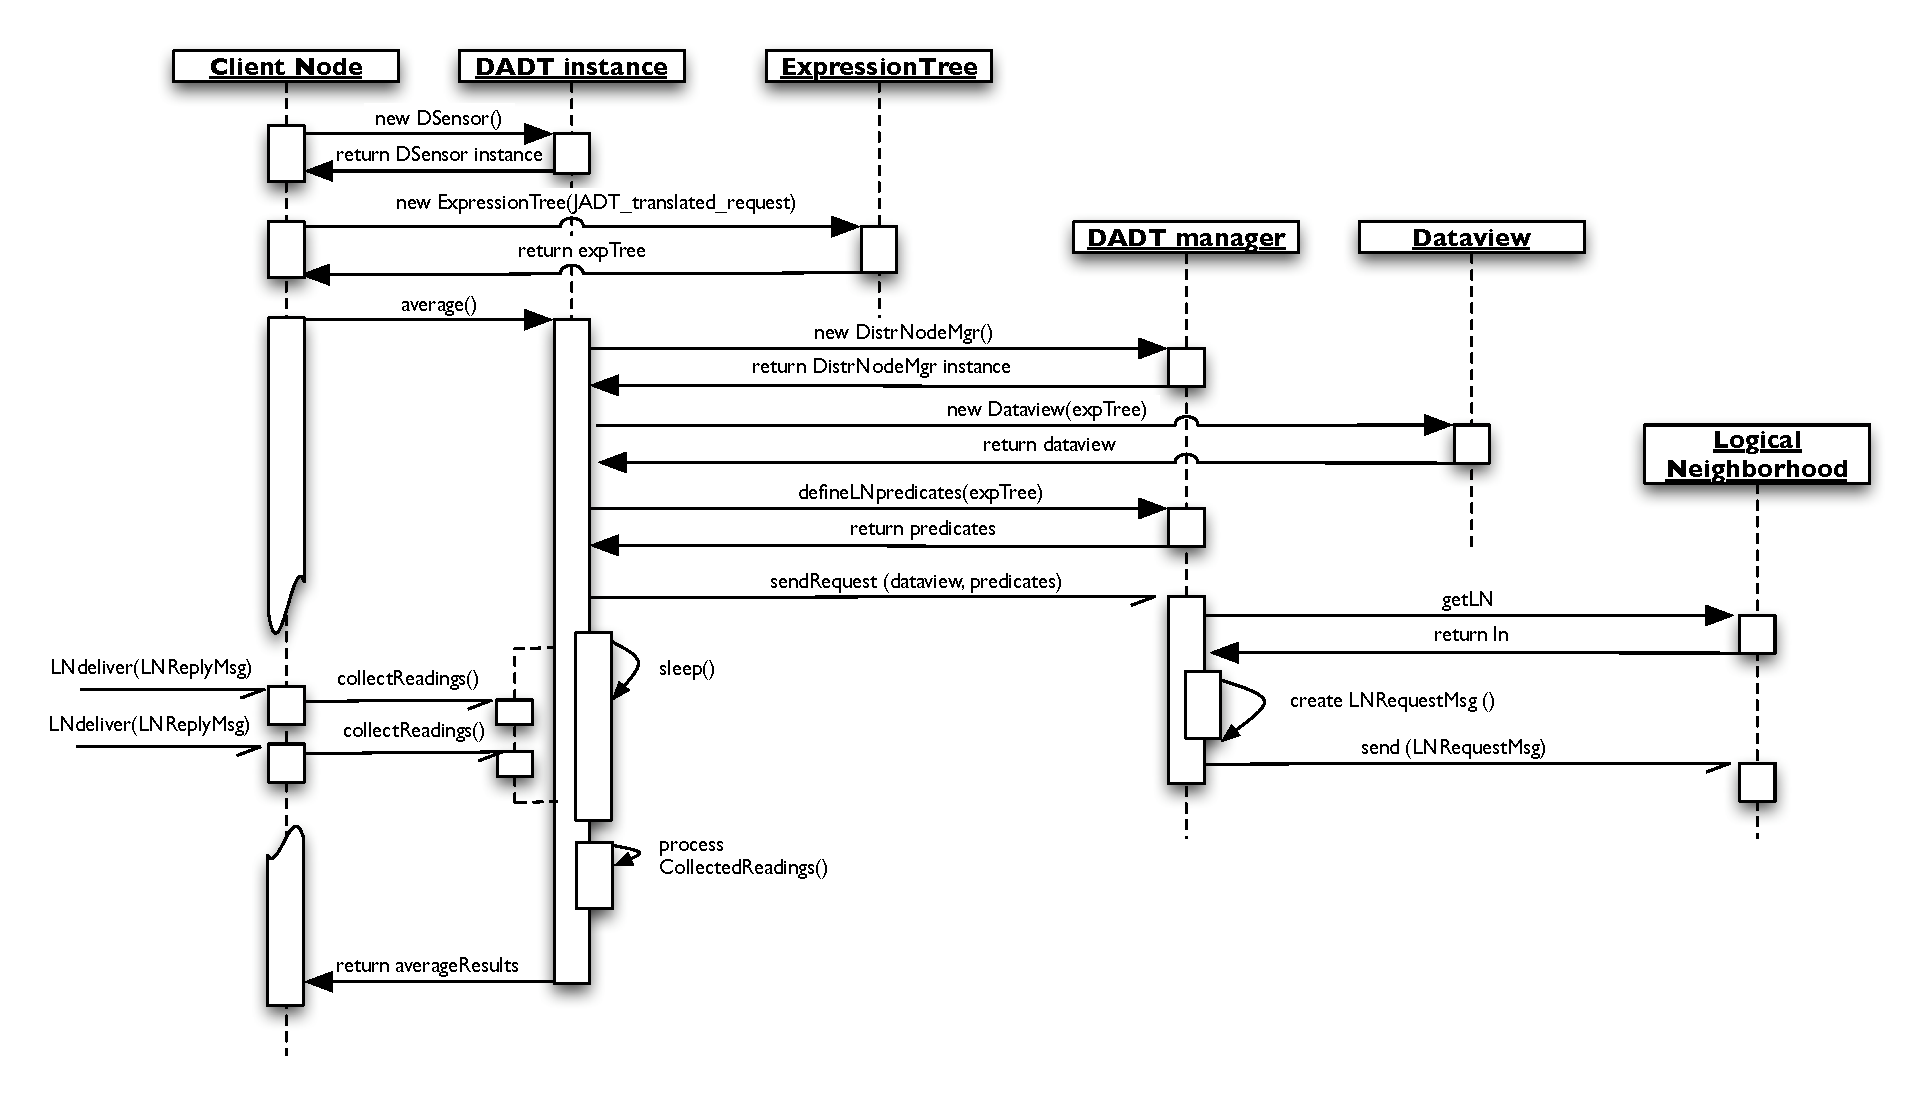
\includegraphics[width=\textwidth]{img/SeqDiagram_PCnode.eps}
\caption[Operation of the DADT/LN prototype on Controller]{Operation of the DADT/LN prototype on Controller}
\label{Fig:SeqDiagram_PCnode}
\end{sidewaysfigure}

\subsection{Workflow}

The instantiation of a DADT type by the application programmer's
code causes the following actions to take place at the Controller:
\begin{itemize}
 \item The Client Node creates an instance of the DADT type and uses it 
 to perform collective operations on the network.
  \item A new expression tree object 
  is created to provide a representation of the DADT View defined by the application
  programmer.
  \item The DADT instance creates an instance of the DistrNode Manager.
\end{itemize}

When the application programmer's code requests the execution of a distributed operation, the Client Node forwards the request to the DADT instance, which in turn
processes the request and facilitates communication across the WSN.

The DADT instance performs the following actions:
  \begin{itemize} 
    \item It processes the request, and, according to the defined scope of the
    distributed operation, constructs the relevant DADT View using the
    expression tree object.
    \item It uses the DistrNode Manager to translate the DADT View
    (defined in the expression tree object) into LN predicates, and constructs and sends a request message to
    the underlying WSN.
    \item The DADT instance sleeps until, if required, the result of
    the request is received from the network layer.
  \end{itemize}
  
If no reply is expected from the nodes to which message was sent, the
Client Node continues to operate normally. This situation occurs, for instance,
in the case of Controller Node requiring each sensor node to execute the \emph{ResetAll} action.
 
Otherwise, if the result of the distributed computation is expected, the DADT
instance is notified when the relevant data are received from the WSN.
The DADT instance then invokes the relevant methods to collect and process the received
readings. Finally, it returns the result of the DADT request to
the Client Node.

\subsection{Interaction between DADT and LN layers} \label{subsec:DADTLNMapping}

The DistrNode Manager is responsible for the interaction between DADT and LN
layers, as was mentioned in Section \ref{subsubsec:LowerLayer}.

Invocation of the request for distributed operation causes the DistrNode Manager
to perform the following actions:
\begin{itemize}
  \item Provide mapping between components of the Expression Tree object, which
  represents the scope of the distributed request and LN predicates.
  \item Identify the required selection operator provided in the request
  (See Section \ref{subsubsec:OperatorsAndActions} for details) and send
  this request to the WSN.
\end{itemize}

Each expresson tree contains a set of DADT Properties, comparison operators
and values associated with each DADT Property. Moreover,
each DADT Property implements method that provides mapping of the DADT
Property into LN predicate by using the relevant LN runtime classes. 

Therefore, when request has to be sent, the DistrNode Manager performs traversal
of the given Expression Tree object and collects a list of LN predicates that
is used later by LN runtime for routing. Listing
\ref{listing:PropertyLNPredicateMapping} presents an example of such a mapping.

\begin{lstlisting}[frame=trbl, basewidth={0.55em, 0.6em}, captionpos=b, 
basicstyle=\ttfamily\footnotesize, breaklines, caption = Mapping DADT Property to LN predicate  label = listing:PropertyLNPredicateMapping]

public class DSensor_isValueLess_Property implements  Property {

  private int valueToCheck;
  private int type;

  public DSensor_isValueLess_Property(int value, int type)  {
    this.valueToCheck = value;
    this.type = type;
  }
  ...
  public Predicate getLNPredicate() {
    return(new IntegerSimplePredicate("value_" + type, IntegerSimplePredicate.LESS_THAN, this.valueToCheck));
  }

  public boolean evaluate(Object o) {
    Sensor local = (Sensor) o;
    if (local.type == type){
      return (local.getSensorReading() < valueToCheck);	
    }
    else 
      return false;
  }
}
\end{lstlisting} 

DADT Property shown in Listing \ref{listing:PropertyLNPredicateMapping}
checks if the sensor of a given type provides a sensor reading which is less than specified by \emph{valueToCheck} field. 
When the request is constructed, method \emph{getLNPredicate} is used and
mapping is performed. 

Currenty the mapping between each DADT Property and relevant LN Predicate
object has to be provided by an application developer manually. Future work may
include implementation of such mapping in automatic mode.

\section{The DADT/LN Prototype on the Sensor Device} \label{subsubsec:DADTLNSensorDevice}

In the rest of this section, the term \emph{sensor device} is used to refer to the
physical sensor node entity, while the term \emph{sensor node} refers to the application
layer abstractions of all of the sensors within the device.

Figure \ref{Fig:SeqDiagram_Sensornode} presents the operation of the DADT/LN
prototype on the sensor device, which may be either a simulated or a Sun SPOT
node.

The DADT/LN prototype implementation running on each sensor node consists of the
following entities:

\begin{itemize}
  \item \emph{Sensor Node} 
  \item \emph{Sensor ADT instance} 
  \item \emph{Node Manager} 
\end{itemize}

A \emph{Sensor Node} is an abstraction that consists of a list of sensors. This
follows from the example used to illustrate the concept of ADTs in Section
\ref{subsec:ADTSpecInst}. 

A \emph{Sensor ADT instance} is the ADT instance of a given sensor on the sensor
node, upon which the prototype executes.

A \emph{Node Manager} provides the interface between the sensor node and the
network, thereby abstracting sensor ADT instances from queries issued by the DADT
instance at the (PC-based) controller.

\begin{sidewaysfigure}[htbp]
\centering
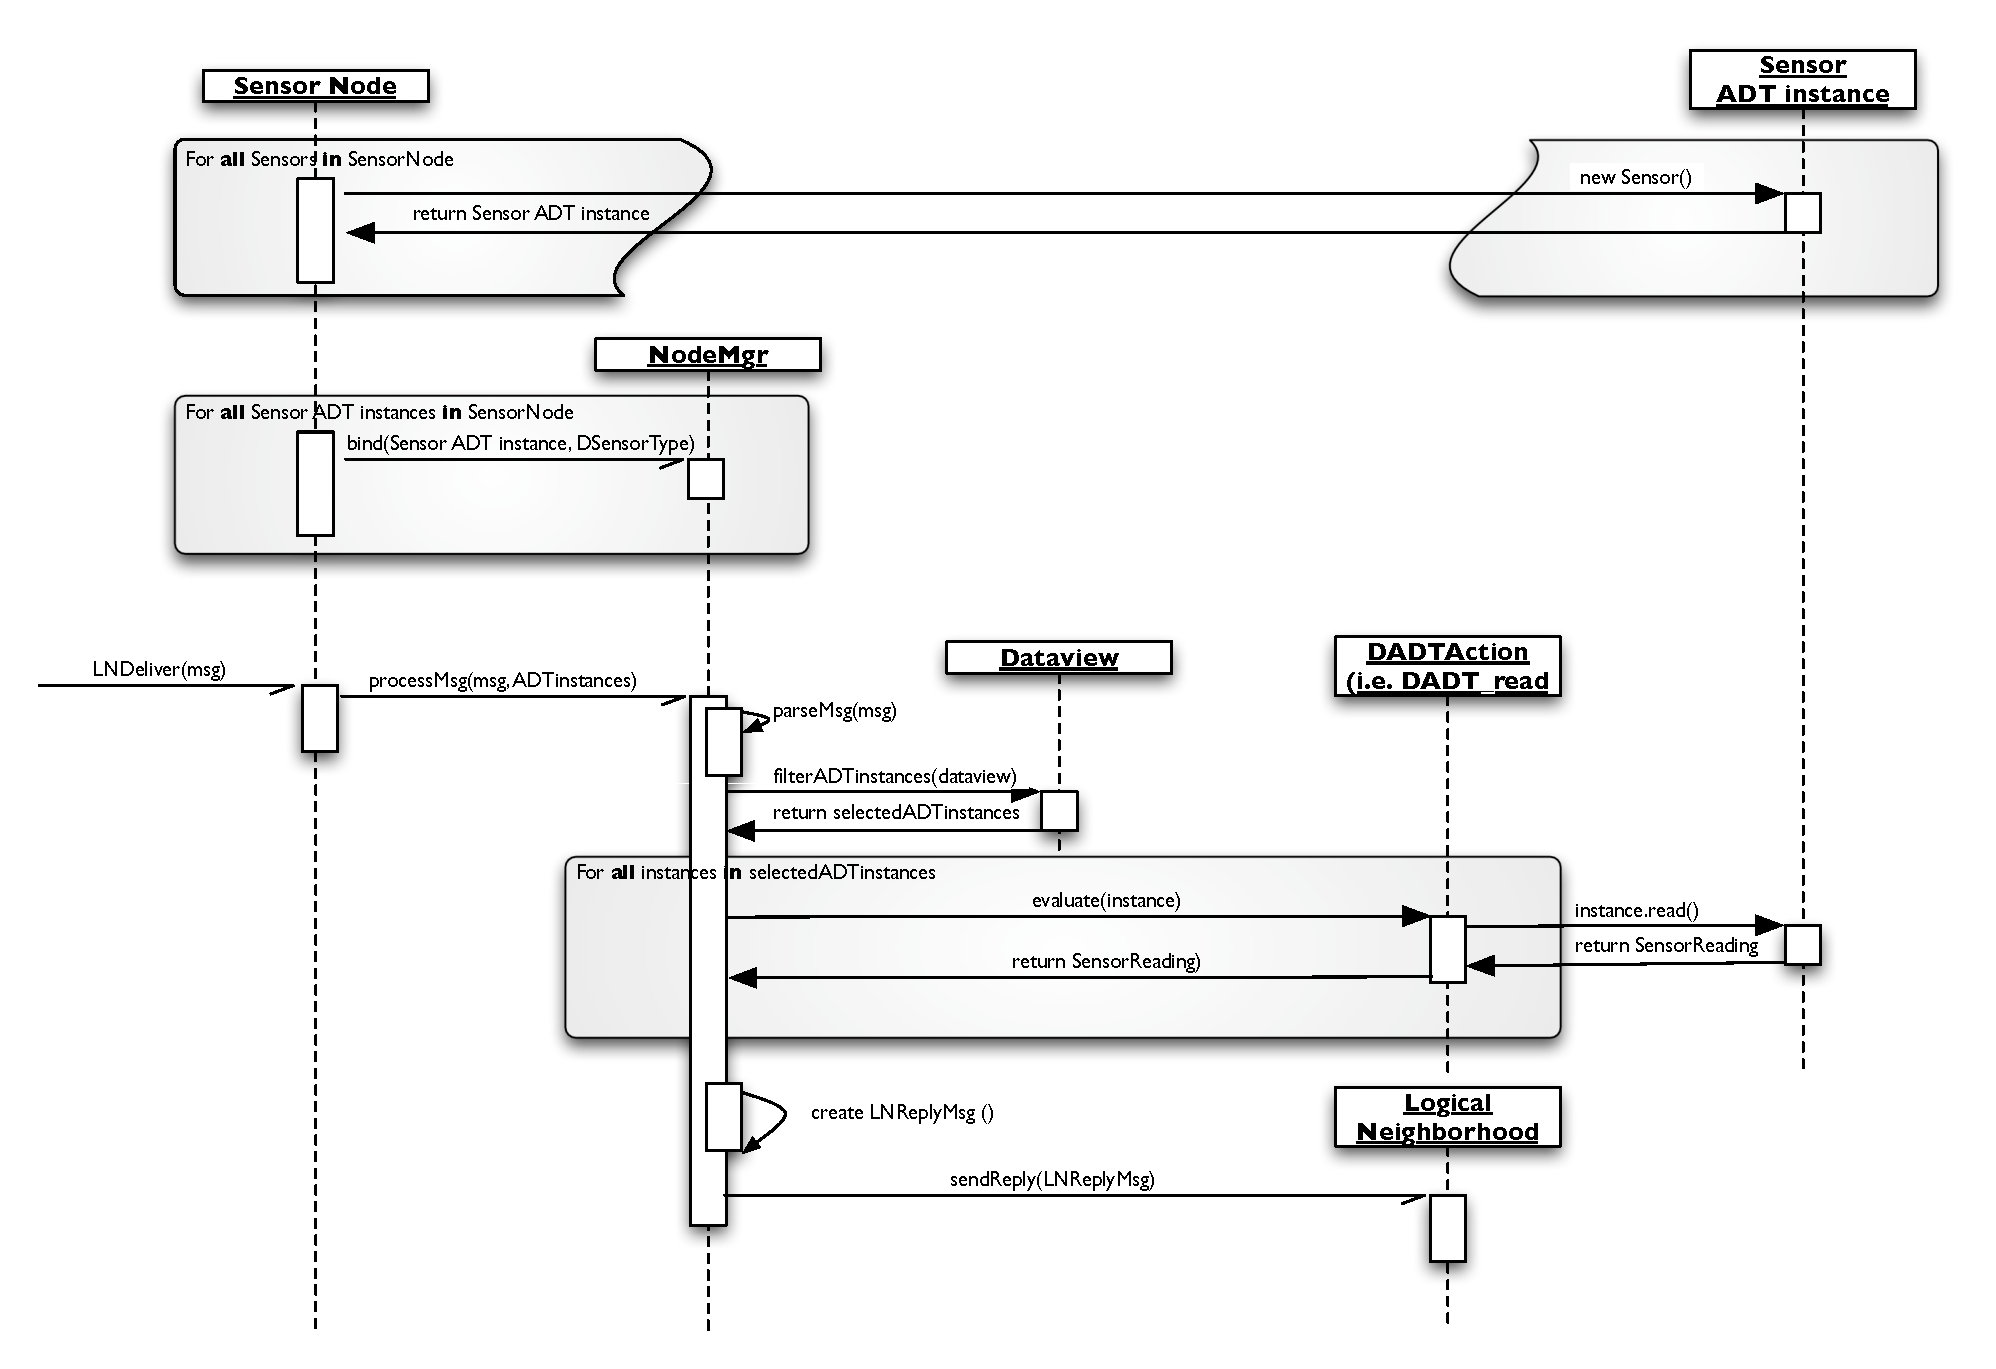
\includegraphics[width=\textwidth]{img/SeqDiagram_Sensornode.eps}
\caption[Operation of the DADT/LN prototype on sensor device]{Operation of the DADT/LN prototype on sensor device}
\label{Fig:SeqDiagram_Sensornode}
\end{sidewaysfigure}

\subsection{Workflow}

Initialisation of the Sensor ADT instance is performed possibly
multiple times on a given Sensor Node, as a node might consist of multiple sensors. Following
this, the sensor ADT instances are bound to a particular DADT type by calling
the Node manager\footnote{The Node manager is assumed in our
current implementation to be aware of all DADT types defined in the WSN.}.

When the lower layer (which runs the LN algorithm) delivers a message to the
Sensor Node, the Node Manager is used to process the request message. The
request message contains details of the DADT View (see Section
\ref{subsubsec:views}) used later to filter from the sensor ADT
instances on the given Sensor node those that fit into the requested DADT View. 

The request message also contains information about the DADT action to be
performed on device (see Section \ref{subsubsec:OperatorsAndActions}). 
The Node manager calls the action for each sensor ADT instance that fits into the DADT View. 

If the application layer requires that a reply be sent, the LN implementation in
the lower layer of the protocol stack is used as can be seen on the bottom
right section of Figure \ref{Fig:SeqDiagram_Sensornode}.

\subsection{Handling of Multiple ADT Instances}

When the request message is received in the application layer, then at least
one of the sensor ADT instances in the Sensor Node fits into the DADT view\footnote{If none of the sensor ADT instances fit the view, the message would have been discarded in the network
layer.}, because LN runtime uses a set of LN predicates based upon DADT view
(See Section \ref{subsec:DADTLNMapping}) for routing. 
This minimises the number of messages received at the application layer. However,
since a given Sensor Node may contain several sensor ADT instances, the ADT
instances have to be filtered.

Filtering is performed by using DADT view object that was sent as the part
of Request message. For each ADT instance binded to the DADT class, all DADT
properties that constitute the DADT view are evaluated. 

Once selection of the relevant for the request ADT instances is done, the
request DADT Action is performed by the \emph{Node Manager}.

\section{Communication Messages} \label{sec:messages}

As was discussed in Chapter \ref{chap:design}, nodes that use the DADT/LN
prototype are communicate between each other by means of specific messages:
\begin{itemize}
  \item \emph{Request message}
  \item \emph{Reply message}
\end{itemize} 

The \emph{Request Message}, as follows from its name, used by controller device
to define a request for distributed action. This message contains 
the following fields: 
\begin{itemize}
  \item \emph{Sender}, which provides information about the node-requestor,
  used later by the sensor device to forward a reply message,
  \item \emph{DADT action}, which specifies the name of the distributed
  action to be executed,
  \item \emph{DADT Classname}, which provides name of the DADT instance,
  \item \emph{DADT View} which represents the scope of the distributed request
  and used by the sensr device to select the relevant  ADT instance.
\end{itemize}

The \emph{Reply Message} used by sensor device to provide the requestor with
relevant sensor data, if it is required. This message contains the following
fields:
\begin{itemize}
  \item \emph{Source}, which specifies the sensor device sending the reply
  \item \emph{Readings}, which stores sensor readings  
\end{itemize}

These messages are sent over WSN and delivered to the nodes by means of LN, as it was discussed in Chapter \ref{chap:design}.

\section{The DADT/LN Prototype in the simulated environment}

\subsection{Simulation using JiST/SWANS}

The DADT/LN prototype was tested on the SWANS WSN simulator, which is built upon
the JiST discrete event simulator (see Section \ref{subsec:jist}). 

The DADT/LN prototype code is wrapped in the JiST API, and is loaded on to a
simulated node. 
The DADT/LN prototype code did not require any changes before depolying
onto simulated nodes due to design of the JiST/SWANS simulator.

As described in the previous section, there are two kinds of
nodes in the DADT/LN prototype:

\begin{itemize}
  \item \emph{Controller Node}, which holds the distributed application, and the
  framework to manage the same.
  \item \emph{Sensor Device}, which holds the individual ADT instances. 
\end{itemize}

The controller node was implemented as a separate node on the JiST/SWANS
simulator and was run as an independent simulated node. The sensor device
implementation (see Section \ref{subsubsec:DADTLNSensorDevice}) was loaded on to all but one of the nodes in
the simulator. Number of nodes in the simulated WSN varied from 30 to 100. 

The controller node was programmed to perform requests for the
distributed operation with a certain periodicity. 
Each sensor device declared 4 different ADT instances of type \emph{Sensor},
e.g. Temperature sensor, Humidity senser, etc., and bound them to the DADT type
\emph{DSensor}. 

The nature of discrete event simulation allowed to verify empirically the
robustness of the prototype done as part of this thesis, but could not provide any evaluation
results relevant for real-world WSNs.

%The simulation was run on networks of up to 50 nodes to develop and
%empirically verify the robustness of the work done as part of this thesis.

\subsection{The DADT/LN Prototype on Sun SPOTs}

For further experimental validation of the implementation produced as part of 
this thesis, the DADT/LN prototype was deployed on Sun SPOTs
\cite{simon_squawk:2006} (see Section \ref{sec:sunspots}).

The Controller application was tested and executed to be run as either:
\begin{itemize}
  \item an on-Host application which communicated with WSN the via basestation node, or 
  \item an on-SPOT application that executed on one of the sensor devices in the WSN, 
\end{itemize}
The other Sun SPOTs ran the Sensor Device implementation as on-SPOT applications
(see Section \ref{subsec:sunspotapps} for a description of host and on-SPOT
applications).

The deployment of the DADT/LN prototype on Sun SPOT devices involved several
challenges. Whereas the JiST/SWANS simulator permits the execution of unmodified Java code
on the simulated node, the Squawk JVM on Sun SPOTs introduces severe limitations
on the code. The application code has to be compliant with the CLDC 1.1 specification
of the Java ME framework, and therefore lacks support for a number of APIs that were
previously used during the development of the DADT prototype \cite{migliavacca_DADT:2006}.

Strict constraints on the supported classes and packages,
e.g. \emph{java.utils}, have required refactoring of the code when deployed
on the Sun SPOT devices. Moreover, lack of support for the serialization of objects resulted in the
necessity to perform serialization ``manually'' for the DADT Action
and the DADT View objects contained in the request messages (see Section
\ref{sec:messages}), and hence, increased size of the request message payload.

\section{Summary}

This chapter presented the details of the implementation of the DADT/LN
prototype developed during the course of this work. The chapter
concluded with a description of the challenges surmounted in order to
further verify the DADT/LN prototype on the Sun SPOT sensor devices.
